%!TEX root = ../../ClassicThesis.tex
% =============================================================================
\section{Introduction}
% =============================================================================


% =============================================================================
\section{Methods}
% =============================================================================

\subsection{Cross-frequency phase-amplitude coupling}

Strength of cross-frequency coupling was measured using the Modulation Index \citep{Tort2010}.
\ac{CSD} data was filtered for two bands, \SIrange{4}{16}{Hz} and \SIrange{60}{170}{Hz}, using a zero-phase sixth-order Butterworth filter, and the instantaneous phase of \SIrange{4}{16}{Hz} and envelope amplitude of \SIrange{60}{170}{Hz} were each estimated using a Hilbert transform.
We took a histogram of the \SIrange{4}{16}{Hz} phase datapoints with \num{16} bins each of width $\nicefrac{\pi}{8}$ radians, and took the average of the \SIrange{60}{170}{Hz} amplitudes simultaneous with the phase datapoints in each bin.
This provides a distribution of amplitude at one depth as a function of phase at another.
The Modulation Index is then the normalised Kullback-Leibler divergence of this distribution from a uniform distribution.


% =============================================================================
\section{Results}
% =============================================================================


%-------------------------------------------------------------------------------
\FloatBarrier
\subsection{Stimulus information contained in phase}

\begin{figure}[htbp]
    \centering
    \hspace*{\fill}
    \subfloat[\ac{LFP}\label{fig:lam_phase_info_lfp}]{
        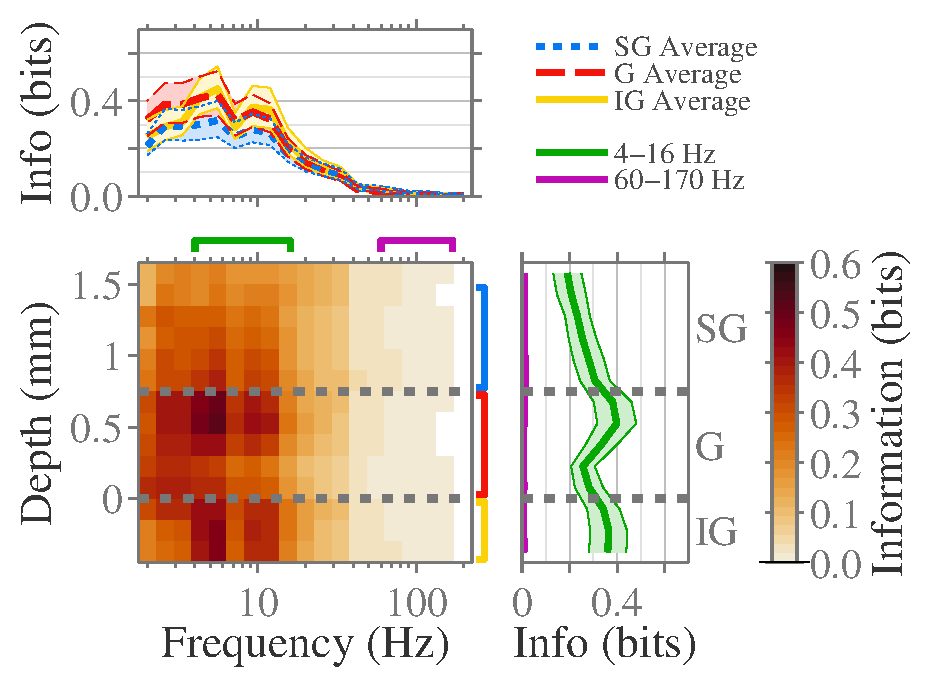
\includegraphics[scale=.45]{phaseinfo/fig3set-info-Csd-phase-straightnanmean-compzonescb-legend.eps}}
    \hspace*{\fill}\hspace{.2cm}\hspace*{\fill}
    \subfloat[\ac{CSD}\label{fig:lam_phase_info_csd}]{
        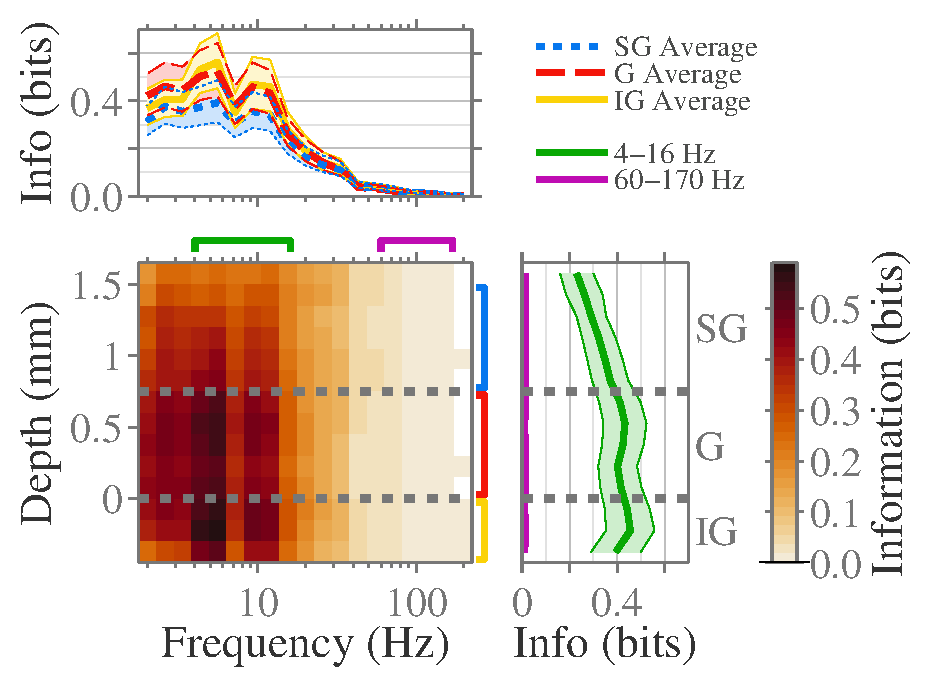
\includegraphics[scale=.45]{phaseinfo/fig3set-info-Cln-phase-straightnanmean-compzonescb-legend.eps}}
    \hspace*{\fill}
    \caption{
Information about the stimulus contained in the phase of the extracellular neural signal, as a function of frequency. Mean of 6 sessions.
\protect\subref{fig:lam_phase_info_lfp}:~\ac{LFP}.
\protect\subref{fig:lam_phase_info_csd}:~\ac{CSD}.
}
\label{fig:lam_phase_info}
\end{figure}


% \begin{figure}[htbp]
%     \centering
%     \hspace*{\fill}
%     \subfloat[\sesname{H05391}\label{fig:lam_phase_info_lfp_H05391}]{
%         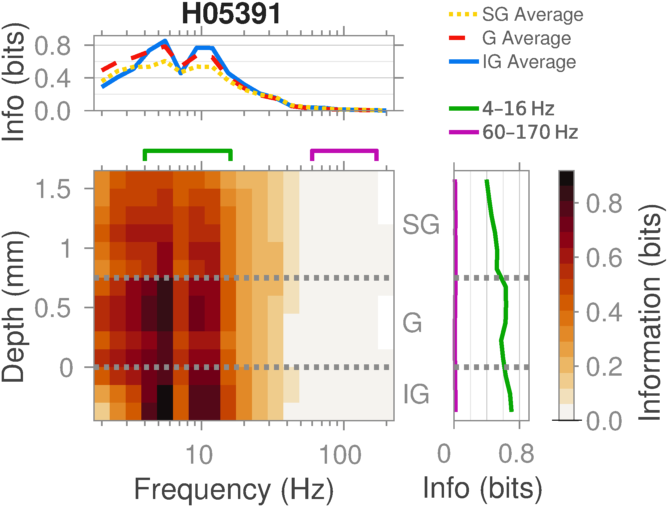
\includegraphics[scale=.4]{phaseinfo/fig3set-info-Cln-phase-H05391-compzonescb-legend.png}
% }
%     \hspace*{\fill}\hspace{.2cm}\hspace*{\fill}
%     \subfloat[\sesname{H05nm9}\label{fig:lam_phase_info_lfp_H05nm9}]{
%         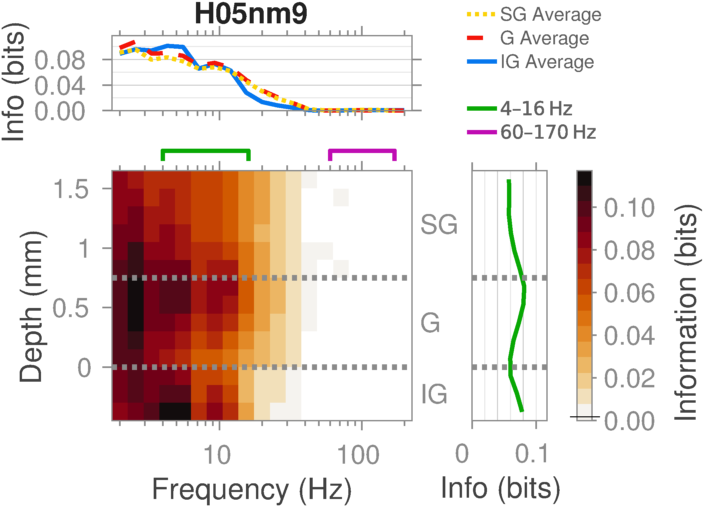
\includegraphics[scale=.4]{phaseinfo/fig3set-info-Cln-phase-H05nm9-compzonescb-legend.png}
% }
%     \hspace*{\fill}
%     \\
%     \hspace*{\fill}
%     \subfloat[\sesname{H05nm7}\label{fig:lam_phase_info_lfp_H05nm7}]{
%         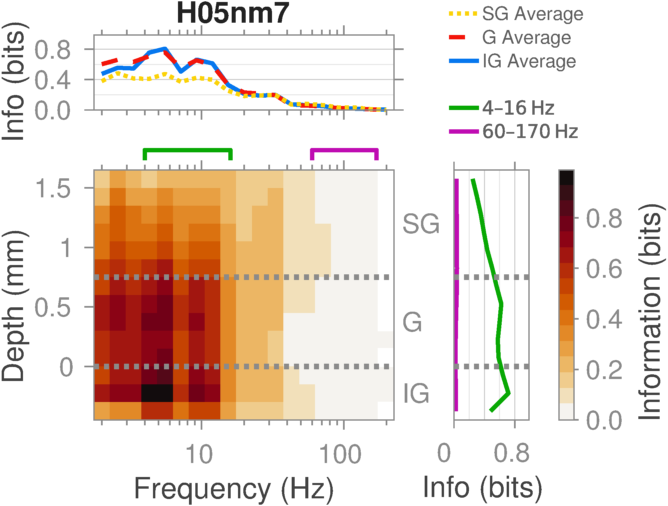
\includegraphics[scale=.4]{phaseinfo/fig3set-info-Cln-phase-H05nm7-compzonescb-legend.png}
% }
%     \hspace*{\fill}\hspace{.2cm}\hspace*{\fill}
%     \subfloat[\sesname{E07nm1}\label{fig:lam_phase_info_lfp_E07nm1}]{
%         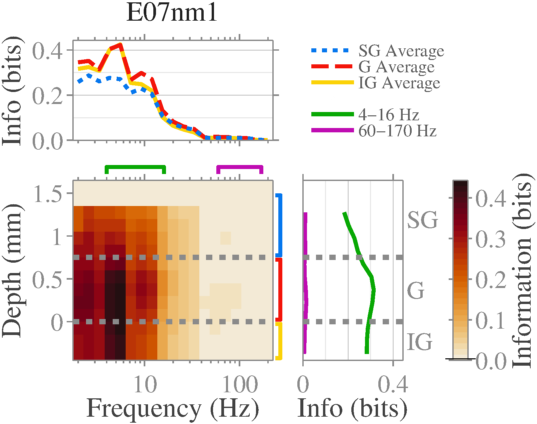
\includegraphics[scale=.4]{phaseinfo/fig3set-info-Cln-phase-E07nm1-compzonescb-legend.png}
% }
%     \hspace*{\fill}
%     \\
%     \hspace*{\fill}
%     \subfloat[\sesname{F10nm1}\label{fig:lam_phase_info_lfp_F10nm1}]{
%         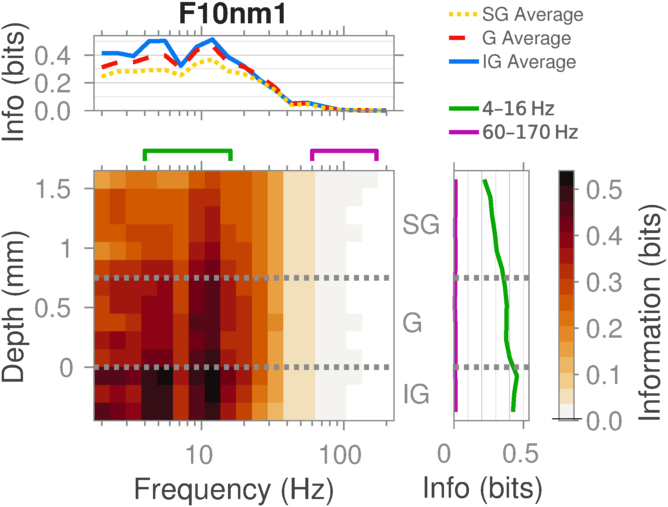
\includegraphics[scale=.4]{phaseinfo/fig3set-info-Cln-phase-F10nm1-compzonescb-legend.png}
% }
%     \hspace*{\fill}\hspace{.2cm}\hspace*{\fill}
%     \subfloat[\sesname{J10nm1}\label{fig:lam_phase_info_lfp_J10nm1}]{
%         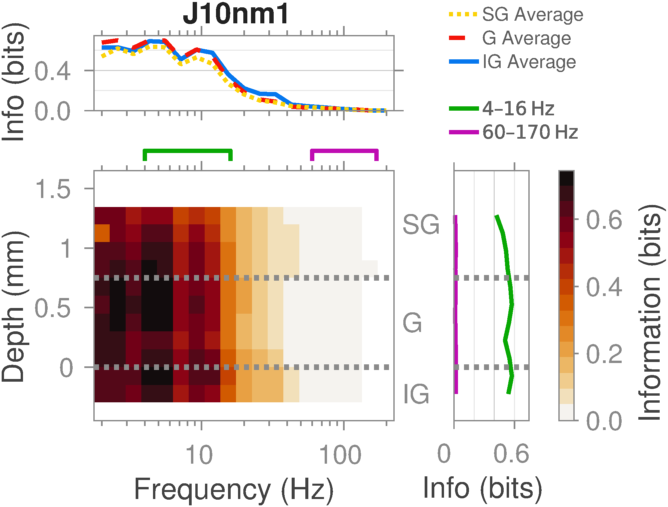
\includegraphics[scale=.4]{phaseinfo/fig3set-info-Cln-phase-J10nm1-compzonescb-legend.png}
% }
%     \hspace*{\fill}
%     \caption{
% Information about the stimulus contained in the phase of the \ac{LFP}, as a function of frequency, by session.
% }
% \label{fig:lam_phase_info_lfp_sessions}
% \end{figure}


% \begin{figure}[htbp]
%     \centering
%     \hspace*{\fill}
%     \subfloat[\sesname{H05391}\label{fig:lam_phase_info_csd_H05391}]{
%         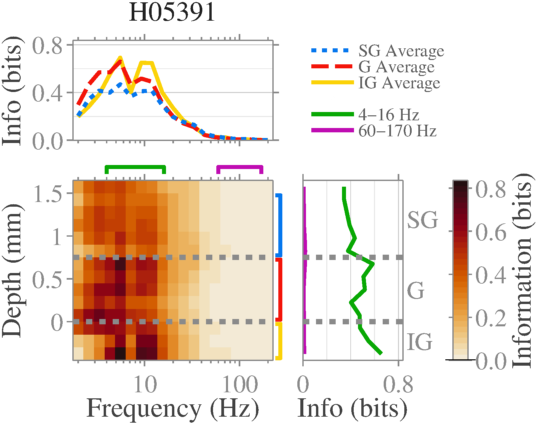
\includegraphics[scale=.4]{phaseinfo/fig3set-info-Csd-phase-H05391-compzonescb-legend.png}
% }
%     \hspace*{\fill}\hspace{.2cm}\hspace*{\fill}
%     \subfloat[\sesname{H05nm9}\label{fig:lam_phase_info_csd_H05nm9}]{
%         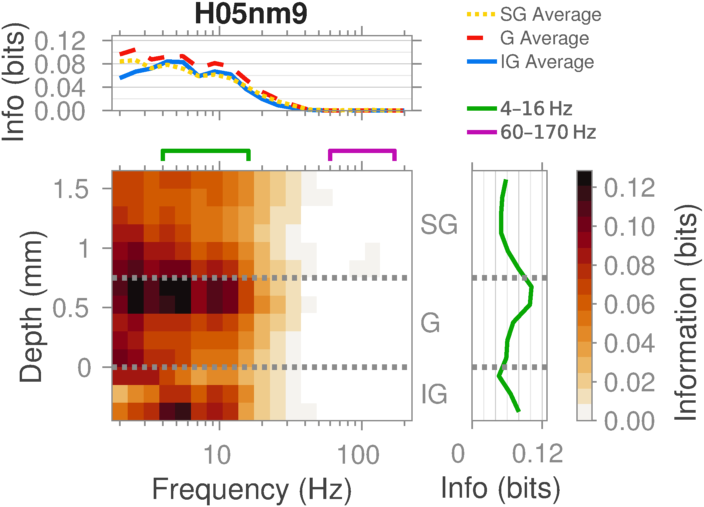
\includegraphics[scale=.4]{phaseinfo/fig3set-info-Csd-phase-H05nm9-compzonescb-legend.png}
% }
%     \hspace*{\fill}
%     \\
%     \hspace*{\fill}
%     \subfloat[\sesname{H05nm7}\label{fig:lam_phase_info_csd_H05nm7}]{
%         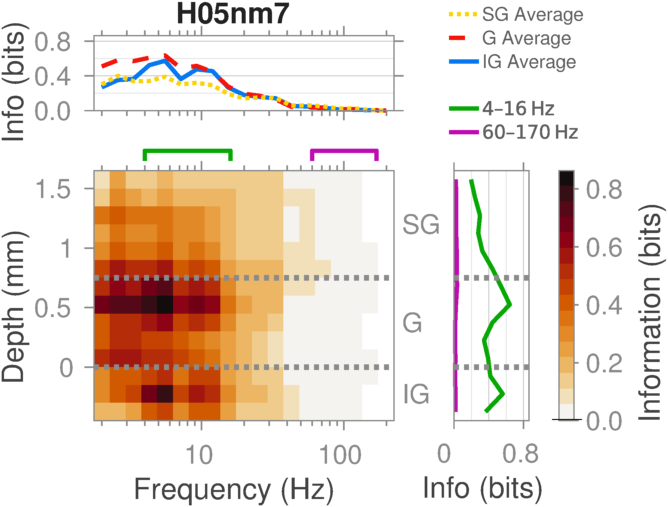
\includegraphics[scale=.4]{phaseinfo/fig3set-info-Csd-phase-H05nm7-compzonescb-legend.png}
% }
%     \hspace*{\fill}\hspace{.2cm}\hspace*{\fill}
%     \subfloat[\sesname{E07nm1}\label{fig:lam_phase_info_csd_E07nm1}]{
%         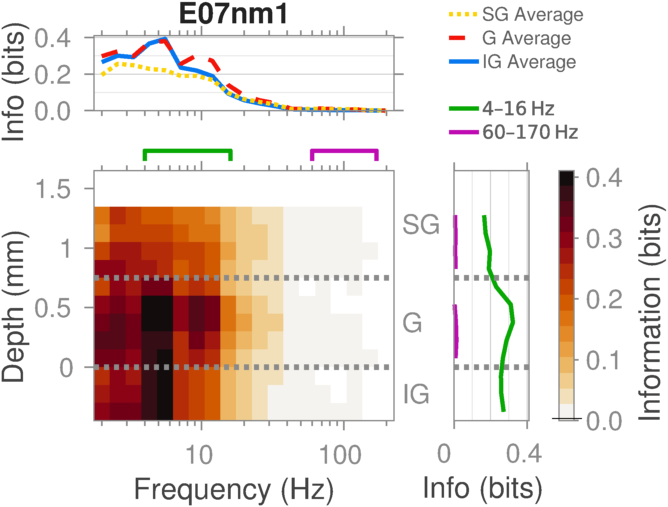
\includegraphics[scale=.4]{phaseinfo/fig3set-info-Csd-phase-E07nm1-compzonescb-legend.png}
% }
%     \hspace*{\fill}
%     \\
%     \hspace*{\fill}
%     \subfloat[\sesname{F10nm1}\label{fig:lam_phase_info_csd_F10nm1}]{
%         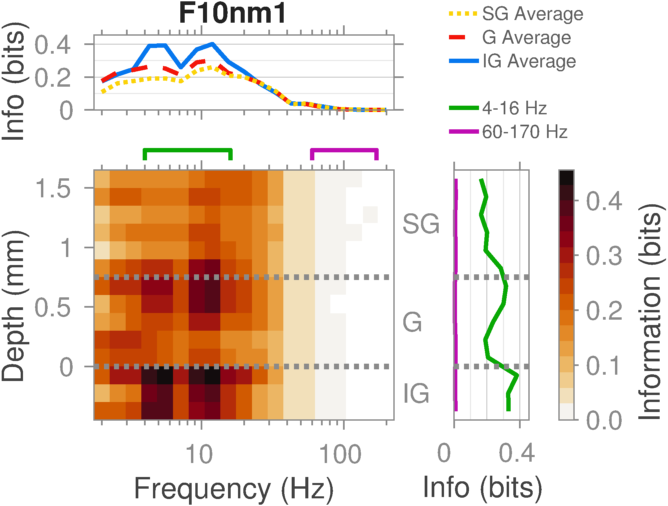
\includegraphics[scale=.4]{phaseinfo/fig3set-info-Csd-phase-F10nm1-compzonescb-legend.png}
% }
%     \hspace*{\fill}\hspace{.2cm}\hspace*{\fill}
%     \subfloat[\sesname{J10nm1}\label{fig:lam_phase_info_csd_J10nm1}]{
%         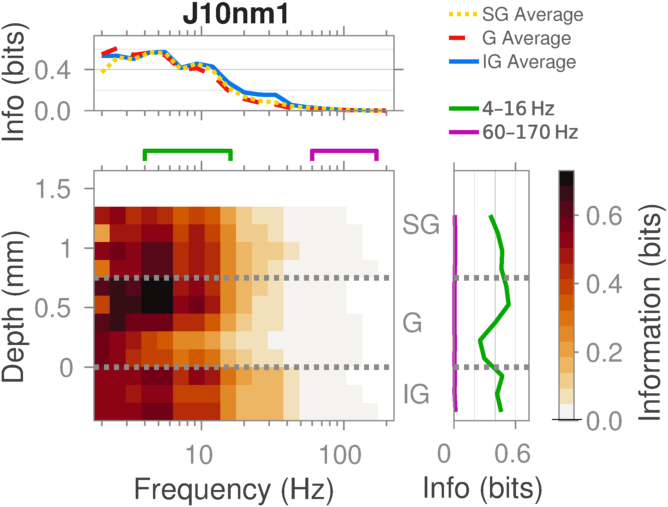
\includegraphics[scale=.4]{phaseinfo/fig3set-info-Csd-phase-J10nm1-compzonescb-legend.png}
% }
%     \hspace*{\fill}
%     \caption{
% Information about the stimulus contained in the phase of the \ac{CSD}, as a function of frequency, by session.
% }
% \label{fig:lam_phase_info_csd_sessions}
% \end{figure}



%-------------------------------------------------------------------------------
\FloatBarrier
\subsection{Redundancy}
%-------------------------------------------------------------------------------

\subsubsection{Cross channel}

\begin{figure}[htbp]
\centering
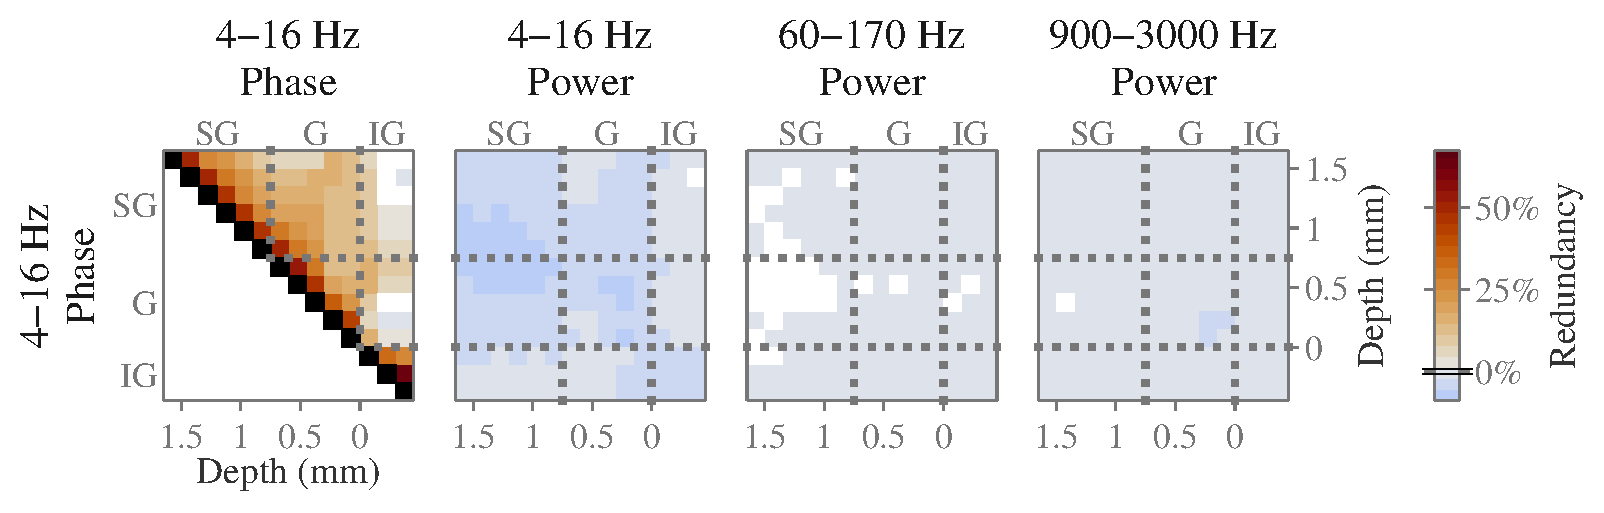
\includegraphics[scale=.5]{redundancy-cxschn/bndflt4-1-pcred-none-avg-lag=0s_paper.eps}
\caption{Redundancy of bands across channels.
}
\label{fig:lam_phase_cxchn_redundancy}
\end{figure}


% \begin{figure}[htbp]
%     \centering
%     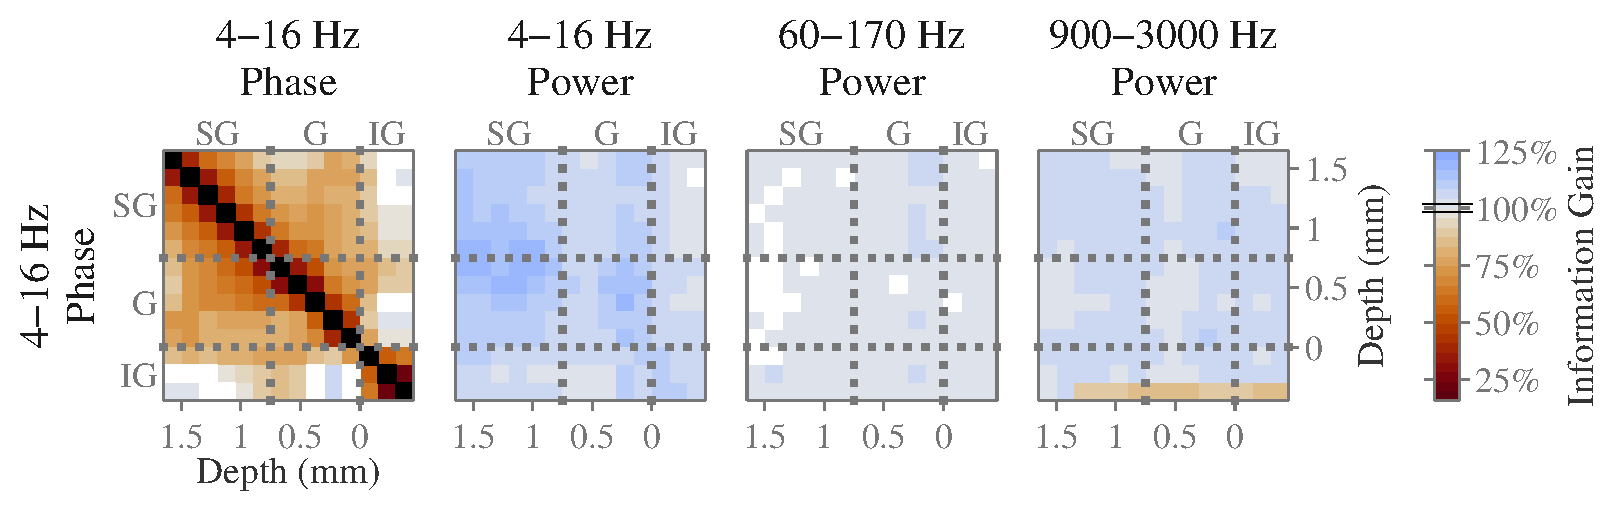
\includegraphics[scale=.5]{redundancy-cxschn/bndflt4-1-pcgain-i2d2-none-avg-lag=0s_paper.eps}
%     \caption{Information gain between bands across channels.
% }
% \label{fig:lam_phase_cxchn_info_gain}
% \end{figure}

% %-------------------------------------------------------------------------------
% \subsubsection{Cross frequency}
%
% \begin{figure}[htbp]
%     \centering
%     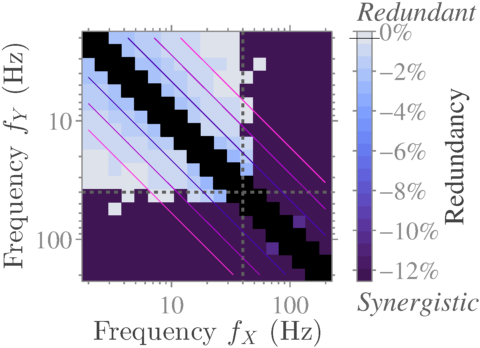
\includegraphics[scale=.5]{redundancy-cxsfrq/cxsfrq-pcred_phase-phase_avg-log}
%     \caption{
% Redundancy between frequencies.
% }
% \label{fig:lam_phase_cxfrq_info_red}
% \end{figure}
%
% \begin{figure}[htbp]
%     \centering
%     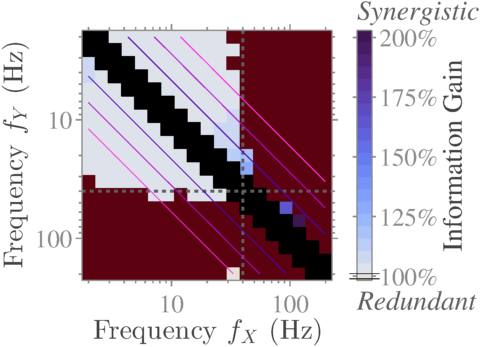
\includegraphics[scale=.5]{redundancy-cxsfrq/cxsfrq-pcgain-i2d2_phase-phase_avg-log}
%     \caption{
% Information gain between frequencies.
% }
% \label{fig:lam_phase_cxfrq_info_gain}
% \end{figure}
%
% %-------------------------------------------------------------------------------
% \subsubsection{Cross frequency phase vs power}
%
% \begin{figure}[htbp]
%     \centering
%     \subfloat[\label{fig:lam_cxfrq_powerphase_info_red_hm}]{
%         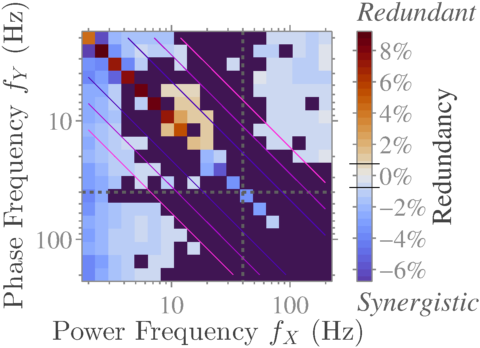
\includegraphics[scale=.5]{redundancy-cxsfrq/cxsfrq-pcred_phase-power_avg-log}
% }
%     \\
%     \subfloat[\label{fig:lam_cxfrq_powerphase_info_red_bar}]{
%         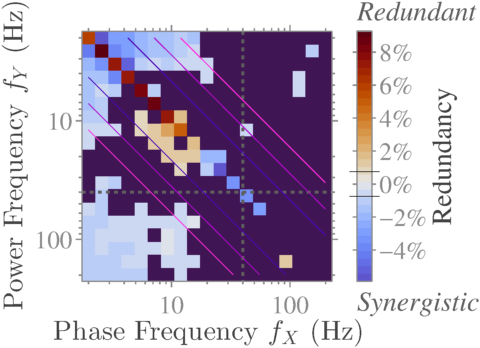
\includegraphics[scale=.5]{redundancy-cxsfrq/cxsfrq-pcred_power-phase_avg-log}
% }
%     \caption{
% Redundancy between frequencies.
% }
% \label{fig:lam_cxfrq_powerphase_info_red}
% \end{figure}
%
%
%
% \begin{figure}[htbp]
%     \centering
%     \subfloat[\label{fig:lam_cxfrq_powerphase_info_gain_hm}]{
%         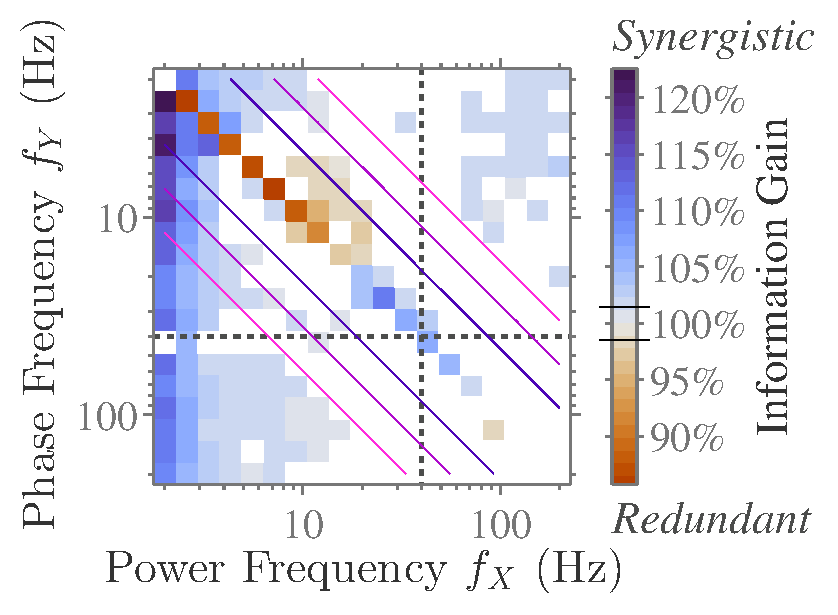
\includegraphics[scale=.5]{redundancy-cxsfrq/cxsfrq-pcgain-i2d2_phase-power_avg-log}
% }
%     \\
%     \subfloat[\label{fig:lam_cxfrq_powerphase_info_gain_bar}]{
%         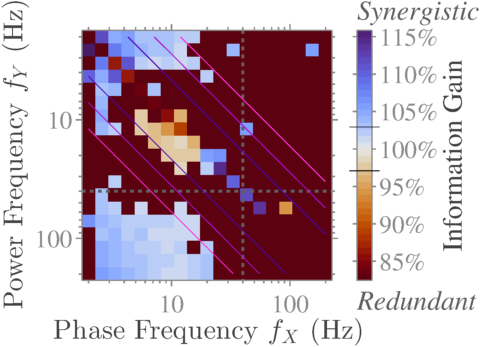
\includegraphics[scale=.5]{redundancy-cxsfrq/cxsfrq-pcgain-i2d2_power-phase_avg-log}
% }
%     \caption{
% Information gain between frequencies.
% }
% \label{fig:lam_cxfrq_powerphase_info_gain}
% \end{figure}
%
%-------------------------------------------------------------------------------
\FloatBarrier
\subsection{Signal and Noise Correlation}

\begin{figure}[htbp]
    \centering
    \subfloat[Signal correlation\label{fig:lam_signal_corr_depth}]{
        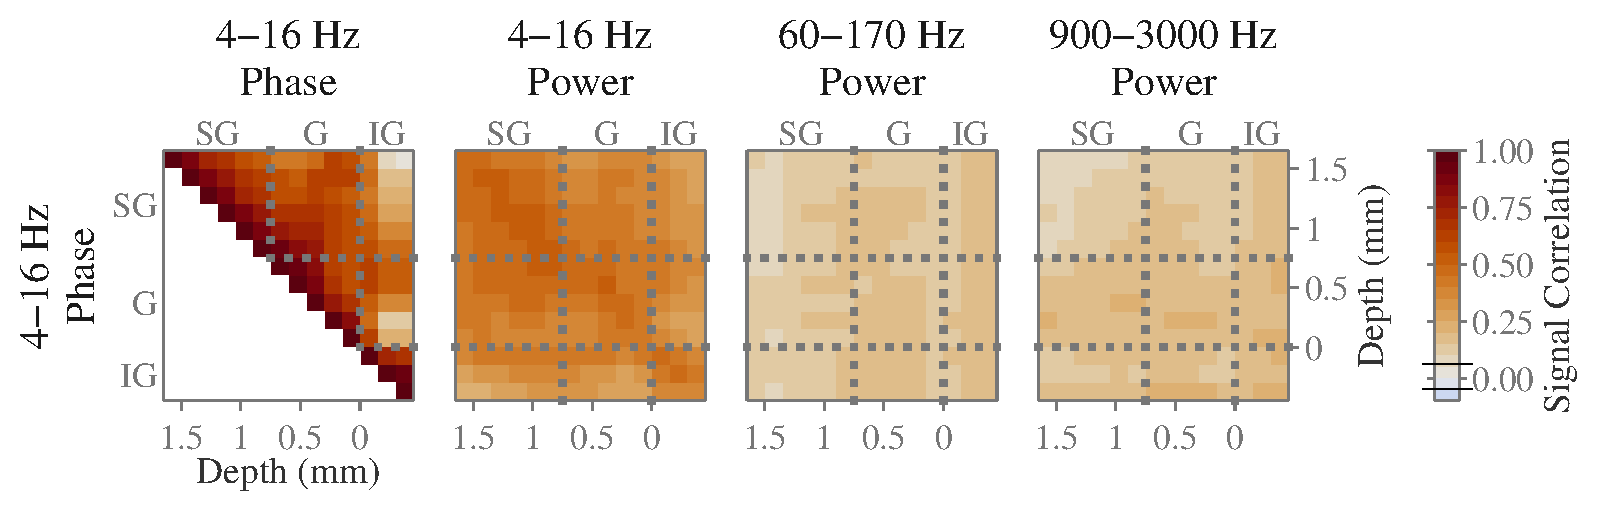
\includegraphics[scale=.5]{noisesigcorr/bndflt4-1-signal-avg_paper.eps}
}
    \\
    \subfloat[Noise correlation\label{fig:lam_noise_corr_depth}]{
        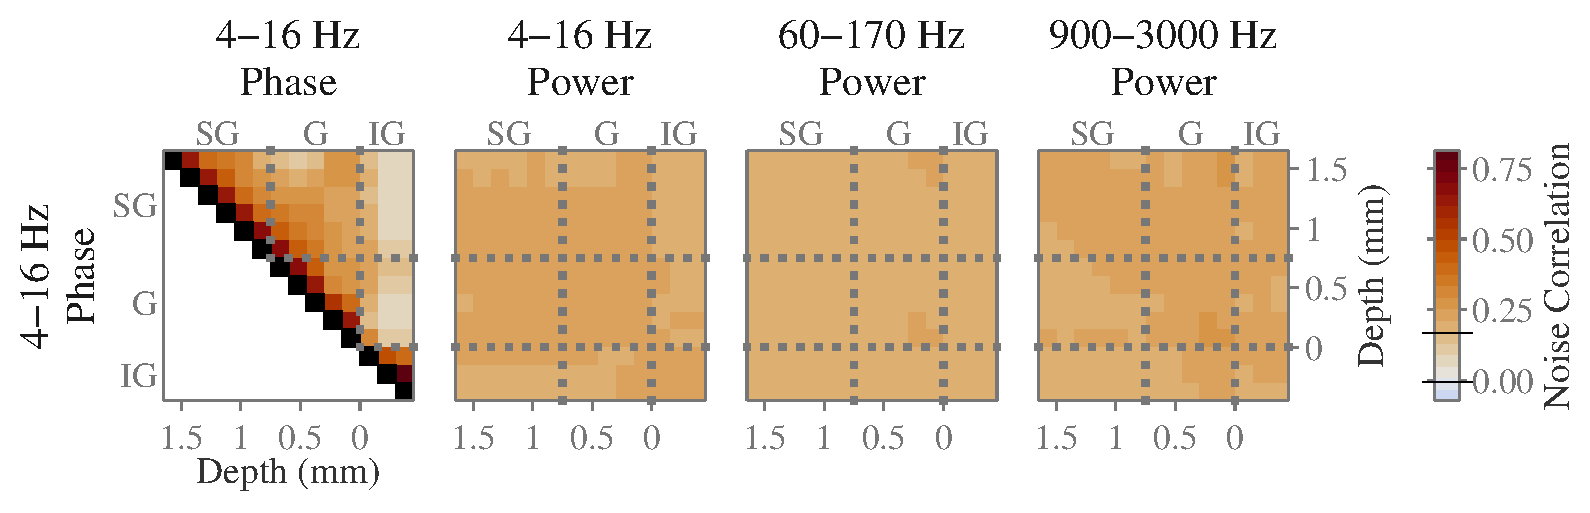
\includegraphics[scale=.5]{noisesigcorr/bndflt4-1-noise-avg_paper.eps}
}
    \caption{
\protect\subref{fig:lam_signal_corr_depth}:~Signal correlation.
\protect\subref{fig:lam_noise_corr_depth}:~Noise correlation.
}
\label{fig:lam_noisesignal_corr_depth}
\end{figure}


\begin{figure}[htbp]
    \centering
    \hspace*{\fill}
    \subfloat[Signal correlation\label{fig:lam_signal_corr_phase}]{
        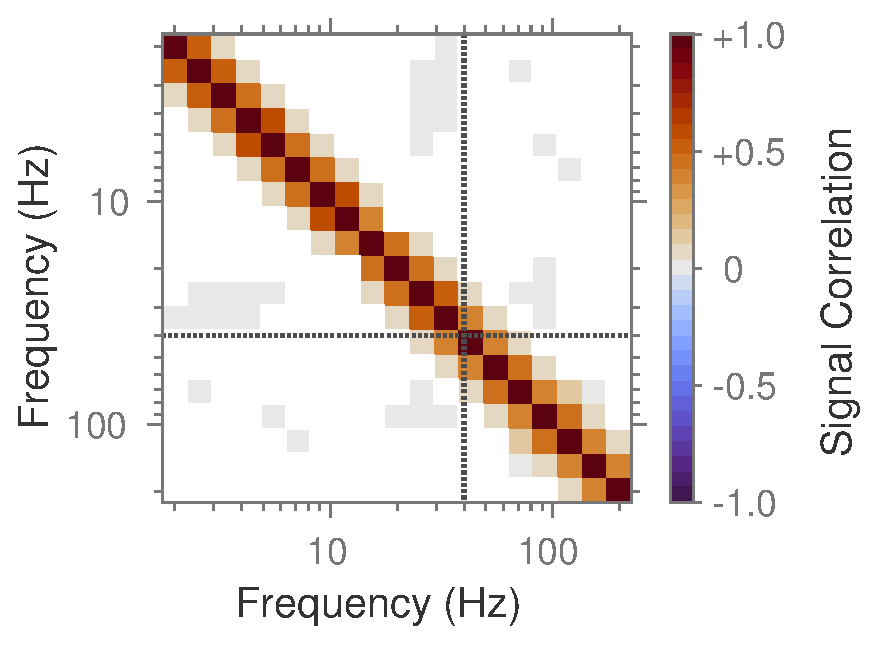
\includegraphics[scale=.45]{noisesigcorr/cxsfrq-signal-phase-phase-avg-log.eps}
}
    \hspace*{\fill}\hspace{.2cm}\hspace*{\fill}
    \subfloat[Noise correlation\label{fig:lam_noise_corr_phase}]{
        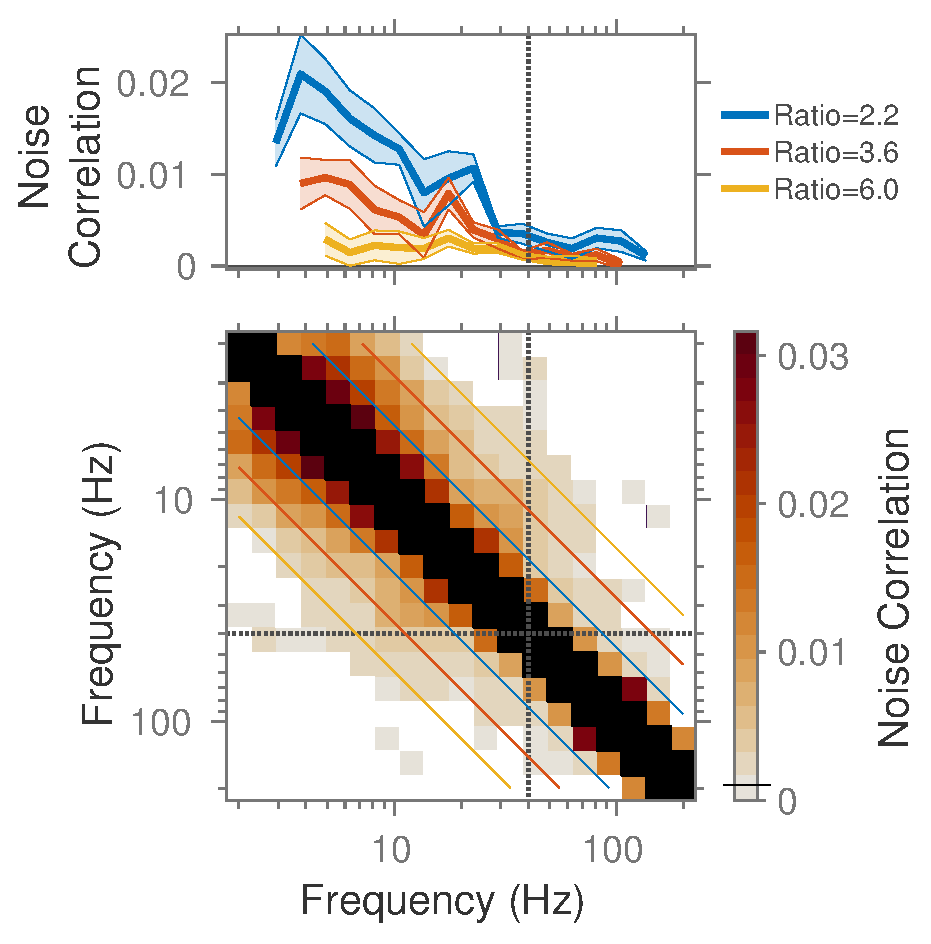
\includegraphics[scale=.45]{noisesigcorr/cxsfrq-noise-phase-phase-avg-log.eps}
}
    \hspace*{\fill}
    \caption{Phase correlation
\protect\subref{fig:lam_signal_corr_phase}:~Signal correlation.
\protect\subref{fig:lam_noise_corr_phase}:~Noise correlation.
}
\label{fig:lam_noisesignal_corr_phase}
\end{figure}

\begin{figure}[htbp]
    \centering
    \hspace*{\fill}
    \subfloat[Signal correlation\label{fig:lam_signal_corr_phase_power}]{
        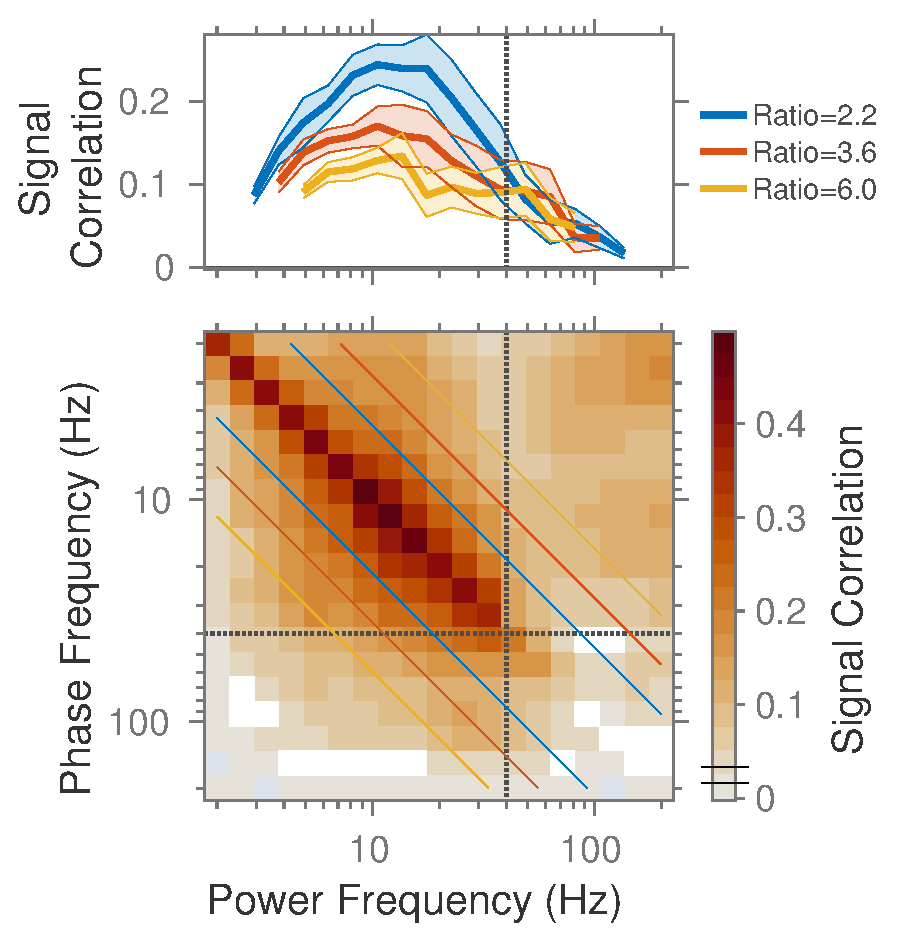
\includegraphics[scale=.45]{noisesigcorr/cxsfrq-signal-phase-power-avg-log.eps}
}
    \hspace*{\fill}\hspace{.2cm}\hspace*{\fill}
    \subfloat[Noise correlation\label{fig:lam_noise_corr_phase_power}]{
        %\includegraphics[scale=.45]{noisesigcorr/cxsfrq-noise-phase-power-avg-log.eps}
        <code running>
}
    \hspace*{\fill}
    \caption{Phase correlation with power
\protect\subref{fig:lam_signal_corr_phase_power}:~Signal correlation.
\protect\subref{fig:lam_noise_corr_phase_power}:~Noise correlation.
}
\label{fig:lam_noisesignal_corr_phase_power}
\end{figure}

Circular statistics were computed using the CircStat toolbox \citep{Berens2009}.

%-------------------------------------------------------------------------------
\FloatBarrier
\subsection{Phase correlation, \SIrange{4}{16}{Hz}}

Circular statistics were computed using the CircStat toolbox \citep{Berens2009}.

\begin{figure}[htbp]
    \centering
    \hspace*{\fill}
    \subfloat[Movie driven\label{fig:lam_phasestats_alpha_line_csd_movie}]{
        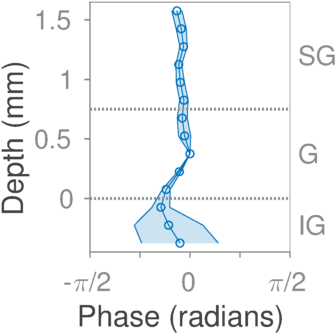
\includegraphics[scale=.45]{phasestats/movie1_Csd_phs4-16_dPhsTracebnd_5mean.png}
}
    \hspace*{\fill}\hspace{.2cm}\hspace*{\fill}
    \subfloat[Spontaneous\label{fig:lam_phasestats_alpha_line_csd_spont}]{
        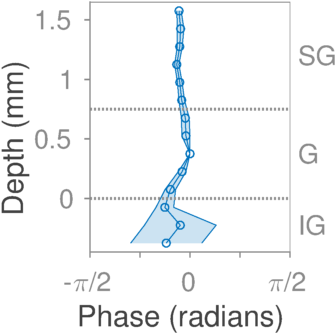
\includegraphics[scale=.45]{phasestats/spont_Csd_phs4-16_dPhsTracebnd_5mean.png}
}
    \hspace*{\fill}
    \caption{Phase correlation, \SIrange{4}{16}{Hz}.
\protect\subref{fig:lam_phasestats_alpha_line_csd_movie}:~Movie driven.
\protect\subref{fig:lam_phasestats_alpha_line_csd_spont}:~Spontaneous.
}
\label{fig:lam_phasestats_alpha_line_csd}
\end{figure}


% \begin{figure}[htbp]
%     \centering
%     \hspace*{\fill}
%     \subfloat[Movie driven\label{fig:lam_phasestats_alpha_hist_csd_movie}]{
%         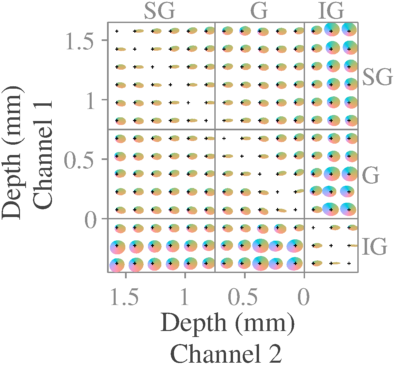
\includegraphics[scale=.45]{phasestats/movie1_Csd_phs4-16_dPhs_hist_5mean.png}
% }
%     \hspace*{\fill}\hspace{.2cm}\hspace*{\fill}
%     \subfloat[Spontaneous\label{fig:lam_phasestats_alpha_hist_csd_spont}]{
%         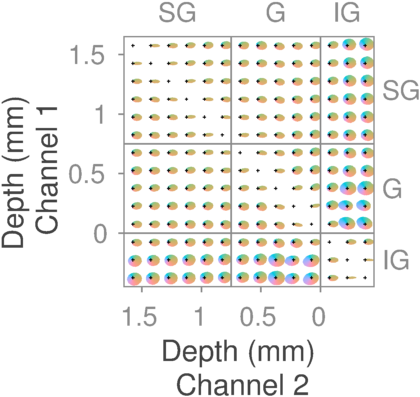
\includegraphics[scale=.45]{phasestats/spont_Csd_phs4-16_dPhs_hist_5mean.png}
% }
%     \hspace*{\fill}
%     \caption{Phase correlation, \SIrange{4}{16}{Hz}.
% \protect\subref{fig:lam_phasestats_alpha_hist_csd_movie}:~Movie driven.
% \protect\subref{fig:lam_phasestats_alpha_hist_csd_spont}:~Spontaneous.
% }
% \label{fig:lam_phasestats_alpha_hist_csd}
% \end{figure}


\begin{figure}[htbp]
    \centering
    \hspace*{\fill}
    \subfloat[Movie driven\label{fig:lam_phasestats_alpha_combo_csd_movie}]{
        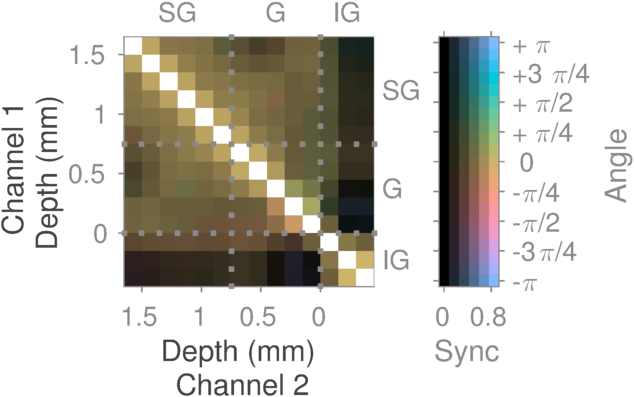
\includegraphics[scale=.45]{phasestats/movie1_Csd_phs4-16_dPhs_combo_5mean.png}
}
    \hspace*{\fill}\hspace{.2cm}\hspace*{\fill}
    \subfloat[Spontaneous\label{fig:lam_phasestats_alpha_combo_csd_spont}]{
        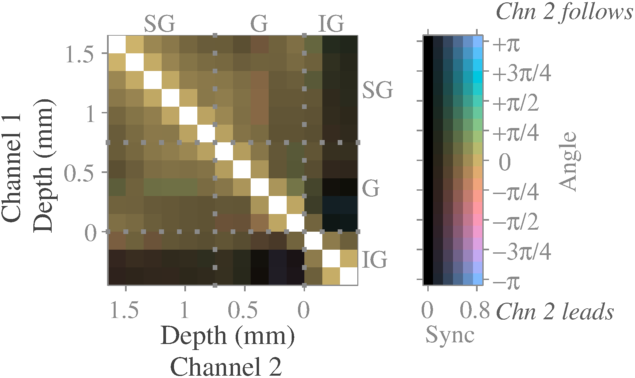
\includegraphics[scale=.45]{phasestats/spont_Csd_phs4-16_dPhs_combo_5mean.png}
}
    \hspace*{\fill}
    \caption{Phase correlation, showing phase offset and synchronicity \SIrange{4}{16}{Hz}.
\protect\subref{fig:lam_phasestats_alpha_combo_csd_movie}:~Movie driven.
\protect\subref{fig:lam_phasestats_alpha_combo_csd_spont}:~Spontaneous.
}
\label{fig:lam_phasestats_alpha_combo_csd}
\end{figure}


\begin{figure}[htbp]
    \centering
    \hspace*{\fill}
    \subfloat[Movie driven\label{fig:lam_phasestats_alpha_summary_csd_movie}]{
        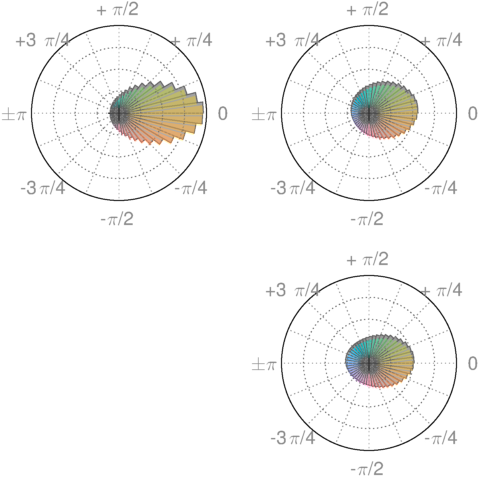
\includegraphics[scale=.45]{phasestats/movie1_Csd_simplephs4-16_dPhs_hist.png}
}
    \hspace*{\fill}\hspace{.2cm}\hspace*{\fill}
    \subfloat[Spontaneous\label{fig:lam_phasestats_alpha_summary_csd_spont}]{
        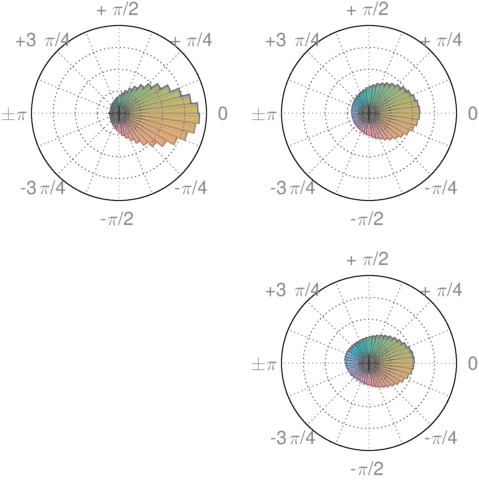
\includegraphics[scale=.45]{phasestats/spont_Csd_simplephs4-16_dPhs_hist.png}
}
    \hspace*{\fill}
    \caption{Phase correlation, summary by region, \SIrange{4}{16}{Hz}.
\protect\subref{fig:lam_phasestats_alpha_summary_csd_movie}:~Movie driven.
\protect\subref{fig:lam_phasestats_alpha_summary_csd_spont}:~Spontaneous.
}
\label{fig:lam_phasestats_alpha_summary_csd}
\end{figure}

%-------------------------------------------------------------------------------
\FloatBarrier
\subsection{Phase correlation, \SIrange{60}{170}{Hz}}

Circular statistics were computed using the CircStat toolbox \citep{Berens2009}.

\begin{figure}[htbp]
    \centering
    \hspace*{\fill}
    \subfloat[Movie driven\label{fig:lam_phasestats_gamma_line_csd_movie}]{
        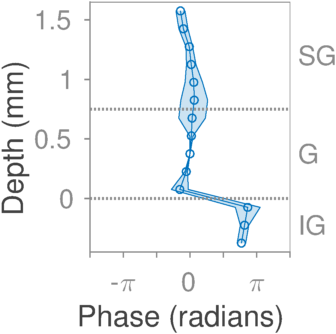
\includegraphics[scale=.45]{phasestats/movie1_Csd_phs60-170_dPhsTracebnd_5mean.png}
}
    \hspace*{\fill}\hspace{.2cm}\hspace*{\fill}
    \subfloat[Spontaneous\label{fig:lam_phasestats_gamma_line_csd_spont}]{
        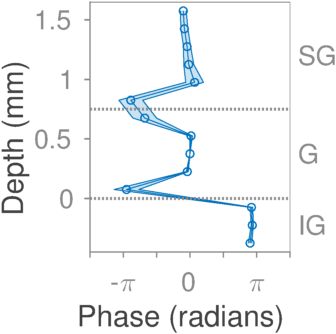
\includegraphics[scale=.45]{phasestats/spont_Csd_phs60-170_dPhsTracebnd_5mean.png}
}
    \hspace*{\fill}
    \caption{Phase correlation, \SIrange{60}{170}{Hz}.
\protect\subref{fig:lam_phasestats_gamma_line_csd_movie}:~Movie driven.
\protect\subref{fig:lam_phasestats_gamma_line_csd_spont}:~Spontaneous.
}
\label{fig:lam_phasestats_gamma_line_csd}
\end{figure}


% \begin{figure}[htbp]
%     \centering
%     \hspace*{\fill}
%     \subfloat[Movie driven\label{fig:lam_phasestats_gamma_hist_csd_movie}]{
%         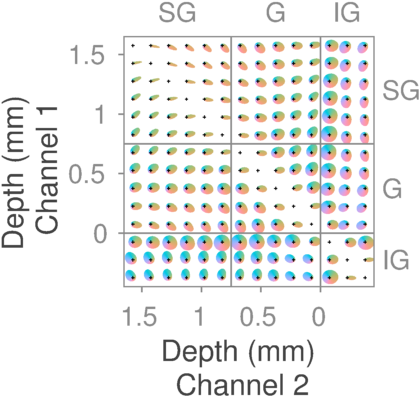
\includegraphics[scale=.45]{phasestats/movie1_Csd_phs60-170_dPhs_hist_5mean.png}
% }
%     \hspace*{\fill}\hspace{.2cm}\hspace*{\fill}
%     \subfloat[Spontaneous\label{fig:lam_phasestats_gamma_hist_csd_spont}]{
%         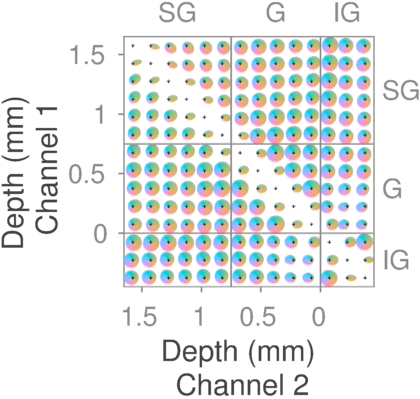
\includegraphics[scale=.45]{phasestats/spont_Csd_phs60-170_dPhs_hist_5mean.png}
% }
%     \hspace*{\fill}
%     \caption{Phase correlation, \SIrange{60}{170}{Hz}.
% \protect\subref{fig:lam_phasestats_gamma_hist_csd_movie}:~Movie driven.
% \protect\subref{fig:lam_phasestats_gamma_hist_csd_spont}:~Spontaneous.
% }
% \label{fig:lam_phasestats_gamma_hist_csd}
% \end{figure}


\begin{figure}[htbp]
    \centering
    \hspace*{\fill}
    \subfloat[Movie driven\label{fig:lam_phasestats_gamma_combo_csd_movie}]{
        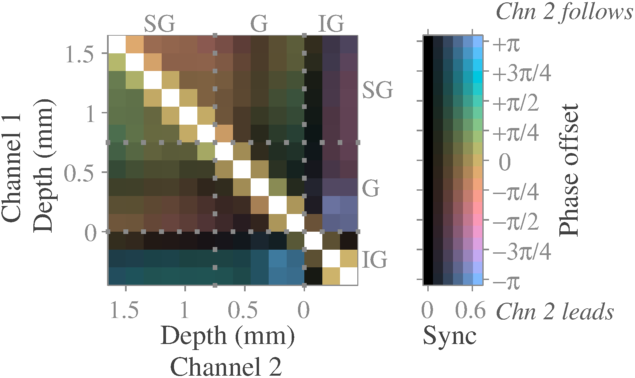
\includegraphics[scale=.45]{phasestats/movie1_Csd_phs60-170_dPhs_combo_5mean.png}
}
    \hspace*{\fill}\hspace{.2cm}\hspace*{\fill}
    \subfloat[Spontaneous\label{fig:lam_phasestats_gamma_combo_csd_spont}]{
        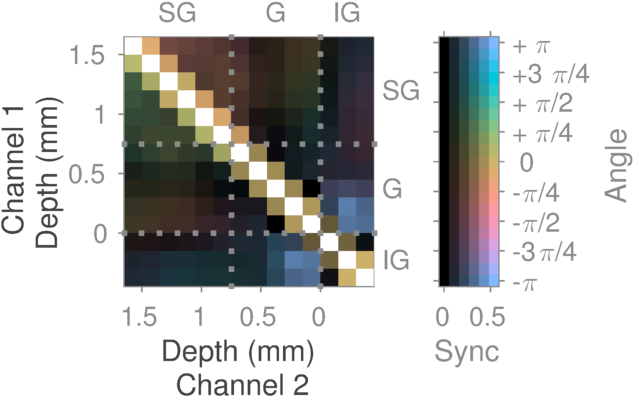
\includegraphics[scale=.45]{phasestats/spont_Csd_phs60-170_dPhs_combo_5mean.png}
}
    \hspace*{\fill}
    \caption{Phase correlation, showing phase offset and synchronicity \SIrange{60}{170}{Hz}.
\protect\subref{fig:lam_phasestats_gamma_combo_csd_movie}:~Movie driven.
\protect\subref{fig:lam_phasestats_gamma_combo_csd_spont}:~Spontaneous.
}
\label{fig:lam_phasestats_gamma_combo_csd}
\end{figure}


\begin{figure}[htbp]
    \centering
    \hspace*{\fill}
    \subfloat[Movie driven\label{fig:lam_phasestats_gamma_summary_csd_movie}]{
        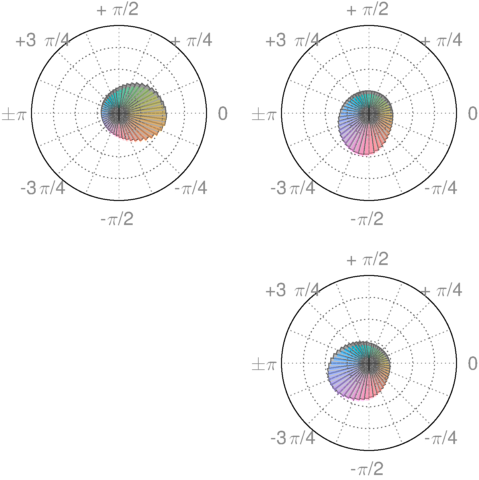
\includegraphics[scale=.45]{phasestats/movie1_Csd_simplephs60-170_dPhs_hist.png}
}
    \hspace*{\fill}\hspace{.2cm}\hspace*{\fill}
    \subfloat[Spontaneous\label{fig:lam_phasestats_gamma_summary_csd_spont}]{
        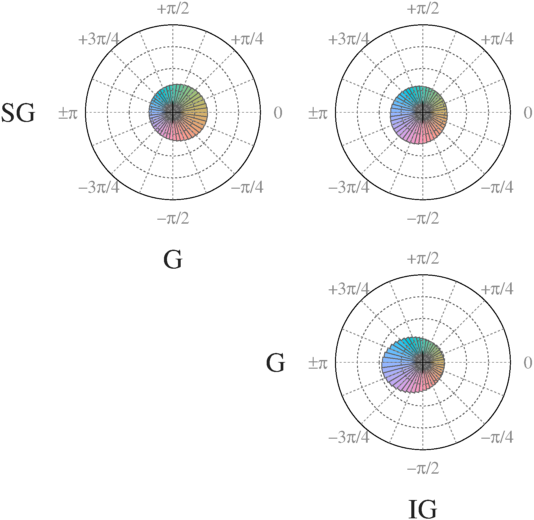
\includegraphics[scale=.45]{phasestats/spont_Csd_simplephs60-170_dPhs_hist.png}
}
    \hspace*{\fill}
    \caption{Phase correlation, summary by region, \SIrange{60}{170}{Hz}.
\protect\subref{fig:lam_phasestats_gamma_summary_csd_movie}:~Movie driven.
\protect\subref{fig:lam_phasestats_gamma_summary_csd_spont}:~Spontaneous.
}
\label{fig:lam_phasestats_gamma_summary_csd}
\end{figure}


\subsection{Layer 1 \SIrange{60}{170}{Hz} amplitude is coupled to L5 \SIrange{4}{16}{Hz} phase}

Above, in section ``Information redundancy across depth'', we showed that high and low \ac{CSD} frequencies contain independent information to each other (\autoref{fig:lam_cxfrq_info}).
We found the power in the two bands to be independent, but it remains possible that there is a relationship between the phase of the low-frequency band and the power of the high-frequency band.
To investigate this possibility, we examined the cross-frequency coupling between the low-frequency phase and high-frequency oscillation amplitude.

Our observations showed that there is a spatially localised coupling between the \SIrange{4}{16}{Hz} phase of both lower-\ac{G} and mid-\ac{IG} with the amplitude of \SIrange{60}{170}{Hz} oscillations in upper-\ac{SG} (\autoref{fig:lam_8}).
Additionally, in both \ac{G} and \ac{IG} there is a coupling between the local \SIrange{4}{16}{Hz} phase and the local \SIrange{60}{170}{Hz} amplitude.

The same relationship was discovered to hold both for spontaneous activity and stimulus-driven recordings, and our findings are in agreement with previous work \citep{Spaak2012}.

\begin{figure}[htbp]
\centering 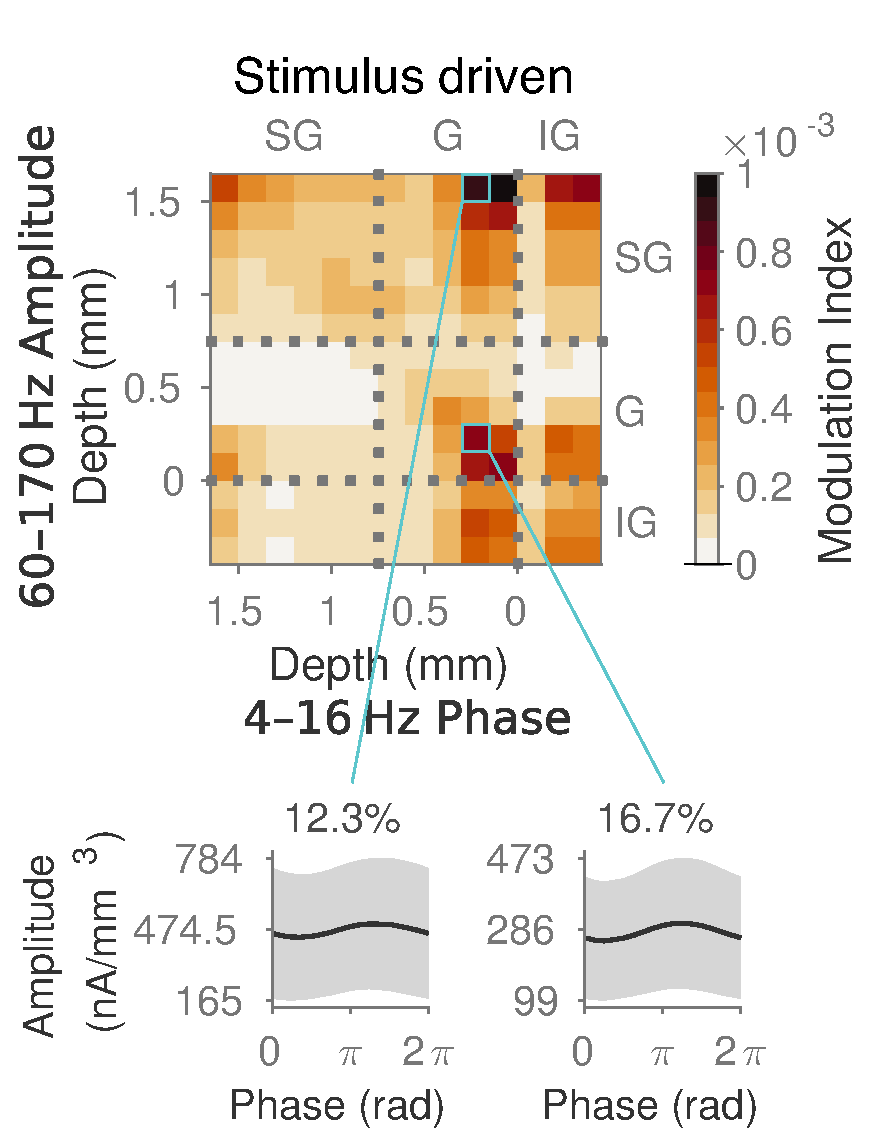
\includegraphics[width=\columnwidth]{cfc/fig8A.eps}
%
\caption{%
\textit{Cross-frequency phase-amplitude coupling}
Phase-amplitude modulation index between low frequency (\SIrange{4}{16}{Hz}) phase and high frequency (\SIrange{60}{170}{Hz}) amplitude (A: movie driven activity; B: spontaneous activity).
Mean of \num{5} sessions.
C and D: Amplitude as a function of binned phase for an example session (\sesname{H05391}), for \ac{IG}$\rightarrow$\ac{IG} coupling (left) and \ac{IG}$\rightarrow$\ac{SG} coupling (right).}%
\label{fig:lam_8}
%
\end{figure}


%-------------------------------------------------------------------------------
\section{Discussion}
%-------------------------------------------------------------------------------
